\section{Finite Volume Method for the Shallow Water Equations}
In this section, we present the finite volume method (FVM) for solving nonlinear systems of balance laws, specifically focusing on the shallow water equations (SWE).
Nonlinear problems are more challenging than linear problems, as stability and convergence theory are more difficult.
Our focus is on discountinuous solutions, that can accurately capture shock waves and other discontinuities.
The approach described here is based on the work of LeVeque~\cite{LeVeque2002}.

In finite volume methods, the computational domain is discretized into cells or control volumes.
At the interfaces between these cells, we solve the local Riemann problem to compute the fluxes.
These fluxes are then used to update the solution in each cell.
By solving the Riemann problem at cell interfaces, the FVM can handle discontinuous solutions, making it particularly well suited for hyperbolic balance laws, such as the shallow water equations.

\subsection{Finite Volume Methods for the 1D SWE}
We begin by considering finite volume methods for the SWE in one space dimension.
In the FVM, we discretize the domain into finite control volumes or cells:
\begin{align*}
    V_i = [x_{i-1/2}, x_{i+1/2}] \times [t_n, t_{n+1}],
\end{align*}
where $\Delta x = x_{i+1/2} - x_{i-1/2}$ is the length of the cell and $\Delta t = t_{n+1} - t_n$ is the time step.
The cell $V_i^n$ is illustrated in Figure~\ref{fig:control_volume_V_i_n}.
\begin{figure}[H]
    \centering
    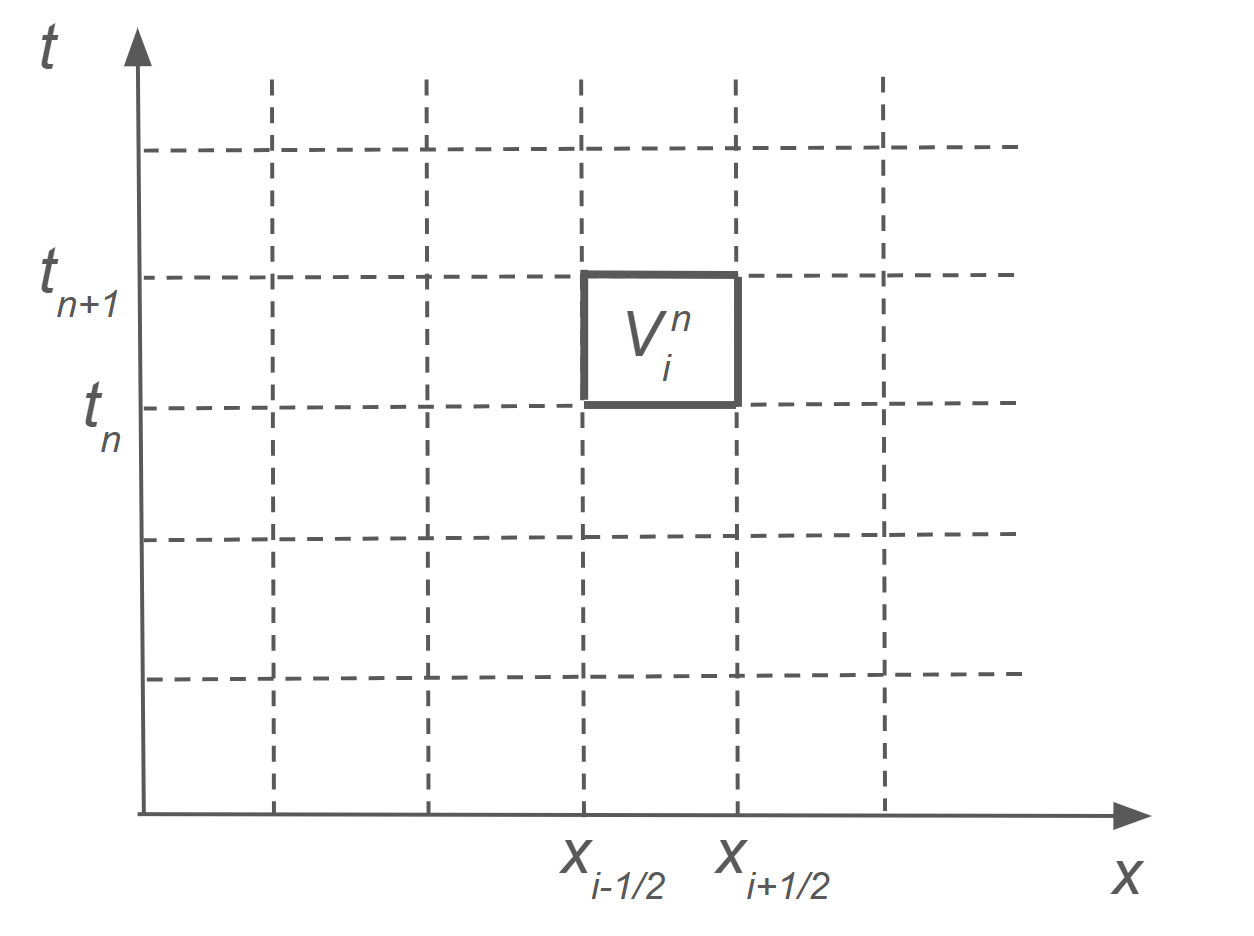
\includegraphics[width=0.4\textwidth]{C:/Users/Matteo/Shallow-Water-Equations/tex/figs/control_volume_V_i_n.png}
    \caption{Illustration of the control volume $V_i^n$ in the $x,t$ plane.}\label{fig:control_volume_V_i_n}
\end{figure}
For now, we will assume a uniform grid for simplicity.
The finite volume formula is derived from the integral form~\eqref{eq:integral_form_1D_final}.
By dividing the integral form of the 1D inhomoegeneous SWE by the cell length $\Delta x$, we espress it in terms of the newly defined cells:
\begin{align*}
    \frac{1}{\Delta x} \int_{x_{i-1/2}}^{x_{i+1/2}} \mathbf{U}(x,t_{n+1}) \text{ d}x &= \frac{1}{\Delta x} \int_{x_{i-1/2}}^{x_{i+1/2}} \mathbf{U}(x,t_n) \text{ d}x\\
    & - \frac{\Delta t}{\Delta x} \left[ \frac{1}{\Delta t} \int_{t_n}^{t_{n+1}} \mathbf{F}(\mathbf{U}(x_{i+1/2}, t)) \text{ d}t
    - \frac{1}{\Delta t} \int_{t_n}^{t_{n+1}} \mathbf{F}(\mathbf{U}(x_{i-1/2}, t)) \text{ d}t \right] \\
    &+ \frac{\Delta t}{\Delta x \Delta t} \int_{x_{i-1/2}}^{x_{i+1/2}} \int_{t_n}^{t_{n+1}} \mathbf{S(U)}(x,t) \text{d}x \text{d}t.
\end{align*}
For a finite volume $V_i^n$, averaging the terms over the volume yields the explicit conservative form
\begin{align}\label{eq:explicit_conservative_1D_SWE}
    \mathbf{U}_i^{n+1} = \mathbf{U}_i^n - \frac{\Delta t}{\Delta x} \left( \mathbf{F}_{i+1/2}^n - \mathbf{F}_{i-1/2}^n \right) + \Delta t \mathbf{S}_i.
\end{align}
The formula~\eqref{eq:explicit_conservative_1D_SWE} is referred to as a finite volume scheme.
The value $\mathbf{U}_i^n$ is the average value over the $i$-th cell at time $t_n$:
\begin{align}
    \mathbf{U}_i^n = \frac{1}{\Delta x} \int_{x_{i-1/2}}^{x_{i+1/2}} \mathbf{U}(x,t_n) \text{ d}x,
\end{align}
also known as the cell average.
The flux $\mathbf{F}_{i-1/2}^n$ is the average flux across the line $x = x_{i-1/2}$ from time $t_n$ to $t_{n+1}$:
\begin{align*}
    \mathbf{F}_{i-1/2}^n = \frac{1}{\Delta t} \int_{t_n}^{t_{n+1}} \mathbf{F}(\mathbf{U}(x_{i-1/2},t)) \text{ d}t,
\end{align*}
and correspondingly the flux $\mathbf{F}_{i+1/2}^n$ is the average flux across the line $x = x_{i+1/2}$ from time $t_n$ to $t_{n+1}$:
\begin{align*}
    \mathbf{F}_{i+1/2}^n = \frac{1}{\Delta t} \int_{t_n}^{t_{n+1}} \mathbf{F}(\mathbf{U}(x_{i+1/2},t)) \text{ d}t.
\end{align*}
The source term $\mathbf{S}_i$ is the average source term over the $i$-th cell at time $t_n$:
\begin{align*}
    \mathbf{S}_i &= \frac{1}{\Delta t \Delta x} \int_{t_n}^{t_{n+1}} \int_{x_{i-1/2}}^{x_{i+1/2}} \mathbf{S}(x,t) \text{ d}x\text{d}t.
\end{align*}
The values are illustrated in Figure~\ref{fig:10_3}.
\begin{figure}[H]
    \centering
    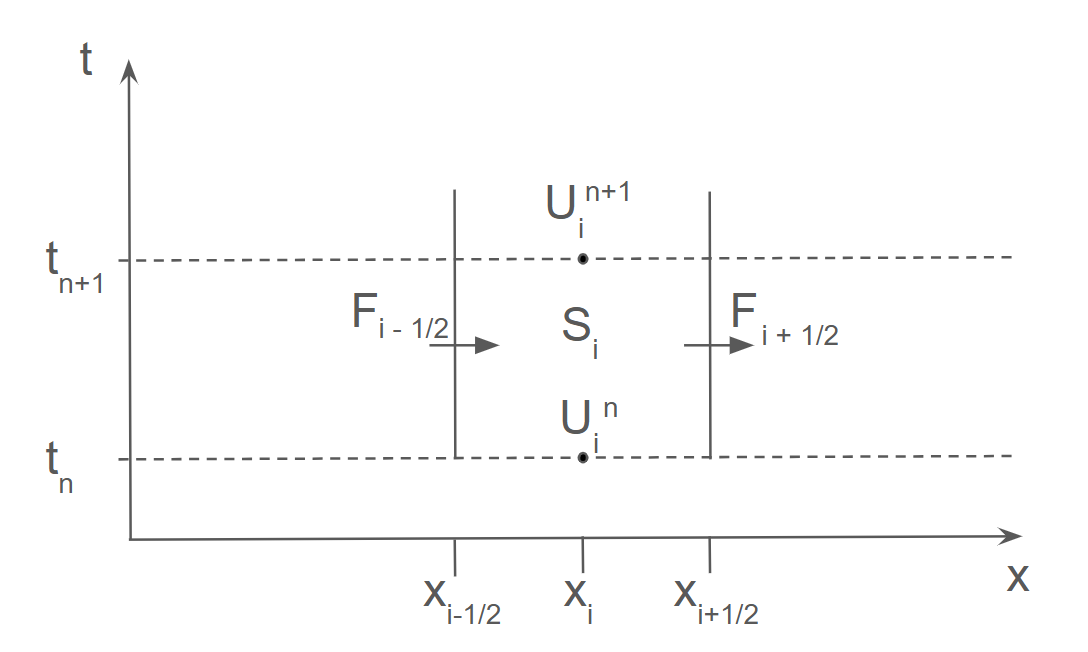
\includegraphics[width=0.5\textwidth]{C:/Users/Matteo/Shallow-Water-Equations/tex/figs/fvm_grid_new.png}
    \caption{Illustration of the grid for the 1D SWE.}\label{fig:10_3}
\end{figure}
The central idea of the FVM is to define the numerical flux $\mathbf{F}_{i+1/2}^n$, at the cell interface, as a function of the cell averages $\mathbf{U}_i^n$ and $\mathbf{U}_{i+1}^n$, since the solution is known only in terms of these cell averages.
Consequently, the FVM does not provide pointwise values of the solution, i.e., $\mathbf{U}(x,t)$, but instead gives cell-averaged values, $\mathbf{U}_i^n$, over the control volume.
One of the main challenges in the FVM is to determine appropiate numerical flux functions that, based on the available cell averages, can reasonably approximate the fluxes at the cell interfaces. 
Later in the thesis, we will consider several numerical flux functions that can be used to solve the local Riemann problem at the cell interfaces.

Finite volume methods are closely related to Finite Difference Methods (FDM), but they differs as they are based on the integral form of the conservation laws.
Where finite difference methods tend to break down near discontinuities in the solution, finite volume methods are more suited, since they are based on the integral form of the conservation laws.
The key distinction between the FVM and the FDM lies in their formulation: while the FVM is based on the integral conservation over finite volumes, the FDM is based on the differential conservation over finite differences.

\subsection{Finite Volume Method for the 2D SWE}
We now extend the FVM to two space dimensions.
Consider the 2D SWE in vector form~\eqref{eq:vector_form_2D} with $\mathbf{S(U)} = 0$:
\begin{align}\label{eq:2D_SWE}
    \mathbf{U}_t + \mathbf{F(U)}_x + \mathbf{G(U)}_y = 0.
\end{align}
Following the methods outlined in~\cite{Toro2009-Riemann}, an explicit finite volume scheme to solve~\eqref{eq:2D_SWE} is given by
\begin{align}
    \mathbf{U}_{i,j}^{n+1} = \mathbf{U}_{i,j}^n + \frac{\Delta t}{\Delta x}(\mathbf{F}_{i-1/2,j} - \mathbf{F}_{i+1/2,j}) + \frac{\Delta t}{\Delta y}(\mathbf{G}_{i,j-1/2} - \mathbf{G}_{i,j+1/2}).
\end{align}
This is the unsplit finite volume method, meaning that, in a single step, the cell average $\mathbf{U}_{i,j}^n$ is updated using the fluxes from all intercell boundaries.


\subsection{Finite Volume Method for the 1D SWE in spherical coordinates}
Simplified linearized shallow water equations on a circle. 
We consider the linearized shallow water equations in cartesian coordinates with one spatial dimension ($x$) and time ($t$).
\begin{equation}
    \left.
    \begin{aligned}
        h_t + H u_x = 0, \\
        u_t + g h_x = 0,
    \end{aligned}
    \right\}
\end{equation}
where $h$ is the height of the water, $u$ is the velocity of the water, $H$ is the average height of the water, and $g$ is the acceleration due to gravity.
We now consider the linearized shallow water equations in spherical coordinates with one spatial dimension, the longitude ($\theta$), and time ($t$).
That is, we assume constant latitude $\phi$. 
As we consider the longitude $\theta$ as the spatial dimension, the domain is the circle $[0, 2\pi]$, which is divided into $N$ cells or control volumes, each of length $\Delta \theta = \frac{2\pi}{N}$.
Each celle $i$ has a cell center at $\theta_i$ and cell boundaries/interfaces at $\theta_{i-1/2}$ and $\theta_{i+1/2}$.
\begin{figure}[H]
    \centering
    \begin{subfigure}{0.4\textwidth}
        \centering
        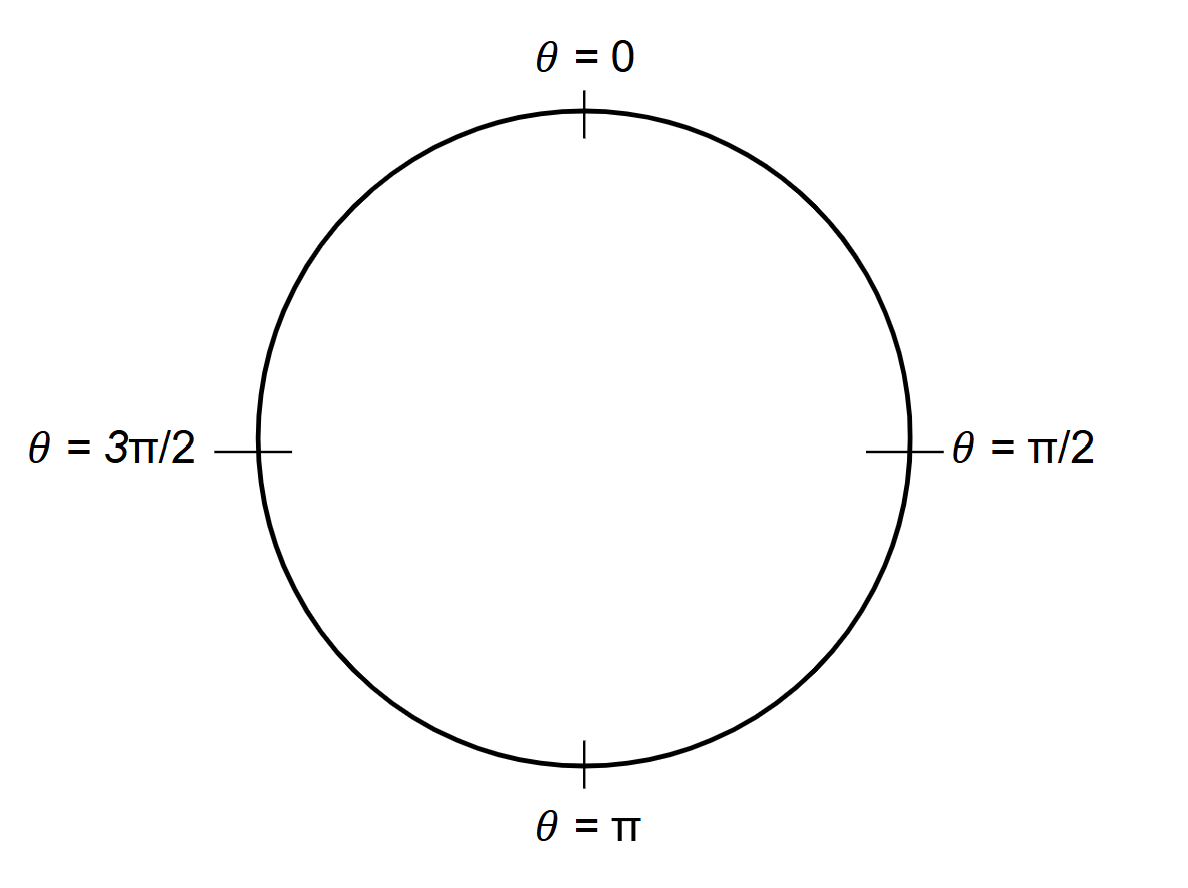
\includegraphics[width=\textwidth]{C:/Users/Matteo/Shallow-Water-Equations/figs/sphere1d_small_cell.png}
        \caption{Illustration of the grid for the 1D SWE with small cells.}\label{fig:sphere1d_small_cell}
    \end{subfigure}%
    \begin{subfigure}{0.35\textwidth}
        \centering
        \raisebox{10mm}{
        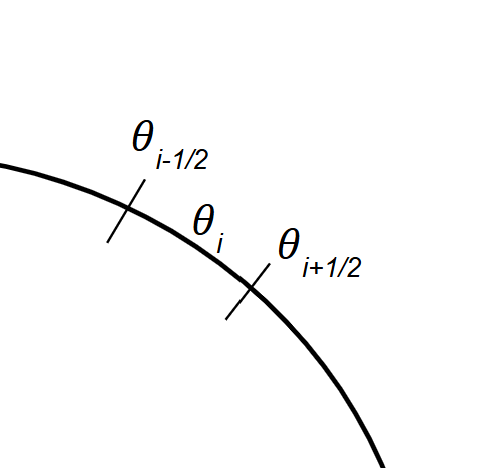
\includegraphics[width=0.9\textwidth]{C:/Users/Matteo/Shallow-Water-Equations/figs/sphere-1d-small-domain.png}
        }
        \caption{Illustration of the grid for the 1D SWE with a small domain.}\label{fig:sphere1d_small_domain}
    \end{subfigure}
    \caption{Grid illustrations for the 1D SWE in spherical coordinates.}\label{fig:sphere1d_combined}
\end{figure}

The linearized shallow water equations in spherical coordinates with one spatial dimension ($\theta$) and time ($t$) are given by
\begin{equation}\label{eq:linearized_swe_spherical}
    \left.
    \begin{aligned}
        h_t + \frac{H}{r \cos(\phi)} u_\theta = 0, \\
        u_t + g h_\theta + fu = 0,
    \end{aligned}
    \right\}
\end{equation}
where $r$ is the radius of the Earth, $\phi$ is the latitude, and $f$ is the Coriolis parameter.
We still refer to the equations as the mass and momentum equations, respectively.
We can also write the linearized shallow water equations in spherical coordinates in vector form, without the coriolis force, as
\begin{align}\label{eq:linearized_swe_spherical_vector}
    \mathbf{W}_t + \mathbf{A} \mathbf{W}_\theta = 0,
\end{align}
where $\mathbf{W} =
\begin{bmatrix} h \\ u \end{bmatrix}$ and the coefficient matrix $\mathbf{A}$ is constant and given as:
$\mathbf{A} = \begin{bmatrix} 0 & \frac{H}{r \cos(\phi)} \\ g & 0 \end{bmatrix}$.
We integrate the height equation in~\eqref{eq:linearized_swe_spherical} over $\theta$ from $\theta_L := \theta_i - \frac{1}{2} \Delta \theta $ to $\theta_R := \theta_i + \frac{1}{2}\Delta \theta $ to obtain
\begin{align*}
    \int_{\theta_L}^{\theta_R} h_t \text{ d}\theta + \int_{\theta_L}^{\theta_R} \frac{H}{r \cos(\phi)} u_\theta \text{ d}\theta = 0.
\end{align*}
The first term is 
\begin{align*}
    \frac{\partial}{\partial t} \int_{\theta_L}^{\theta_R} h \text{ d}\theta =  \Delta \theta h_t,
\end{align*}
meaning that the first term is the rate of change of the water height $h$ in the control volume.
The second term is
\begin{align*}
    \int_{\theta_L}^{\theta_R} \frac{H}{r \cos(\phi)} u_\theta \text{ d}\theta = \frac{H}{r \cos(\phi)} (u_R - u_L),
\end{align*}
where $u_R$ and $u_L$ are the velocities at the right and left boundaries of the control volume, respectively.
Then we integrate the momentum equation in~\eqref{eq:linearized_swe_spherical} over $\theta$ from $\theta_L$ to $\theta_R$ to obtain
\begin{align*}
    \int_{\theta_L}^{\theta_R} u_t \text{ d}\theta + \int_{\theta_L}^{\theta_R} g h_\theta \text{ d}\theta + \int_{\theta_L}^{\theta_R} fu \text{ d} \theta = 0.
\end{align*}
The first term gives the time rate of change in the velocity $u$ in the control volume:
\begin{align*}
    \frac{\partial}{\partial t} \int_{\theta_L}^{\theta_R} u \text{ d}\theta = \Delta \theta u_t.
\end{align*}
The second term gives 
\begin{align*}
    \int_{\theta_L}^{\theta_R} g h_\theta \text{ d}\theta = g(h_R - h_L),
\end{align*}
where $h_R$ and $h_L$ are the heights at the right and left boundaries of the control volume, respectively.
The third term with the Coriolis force gives
\begin{align*}
    \int_{\theta_L}^{\theta_R} fu \text{ d}\theta = f(u_R - u_L) \Delta \theta.
\end{align*} 
Hence, the integral form of the linearized shallow water equations in spherical coordinates with one spatial dimension and time is
\begin{equation}\label{eq:integral_form_spherical_1D}
    \left.
    \begin{aligned}
        \frac{\partial}{\partial t} \int_{\theta_L}^{\theta_R} h \text{ d}\theta + \frac{H}{r \cos(\phi)} (u_R - u_L) &= 0, \\
        \frac{\partial}{\partial t} \int_{\theta_L}^{\theta_R} u \text{ d}\theta + g(h_R - h_L) + fu_i &= 0.
    \end{aligned}
    \right\}
\end{equation}
Then we integrate~\eqref{eq:integral_form_spherical_1D} over time from $t_1:= t_n$ to $t_2:= t_{n+1}$:
\begin{equation}
    \begin{aligned}
        \int_{t_1}^{t_2} \int_{\theta_L}^{\theta_R} h_t \text{ d}\theta \text{d}t + \int_{t_1}^{t_2} \frac{H}{r \cos(\phi)} (u_R - u_L) \text{ d}t &= 0, \\
        \int_{t_1}^{t_2} \int_{\theta_L}^{\theta_R} u_t \text{ d}\theta \text{d}t + \int_{t_1}^{t_2} g(h_R - h_L) \text{ d}t + \int_{t_1}^{t_2} f(u_R - u_L) \Delta \theta &= 0.
    \end{aligned}
\end{equation}
which equals
\begin{equation}\label{eq:integral_form_spherical_1D_2}
    \begin{aligned}
        \int_{\theta_L}^{\theta_R} h(\theta, t_2) \text{ d}\theta &= \int_{\theta_L}^{\theta_R} h(\theta, t_1) \text{ d}\theta - \frac{H}{r \cos(\phi)} (u_R - u_L) \Delta t, \\
        \int_{\theta_L}^{\theta_R} u(\theta, t_2) \text{ d}\theta &= \int_{\theta_L}^{\theta_R} u(\theta, t_1) \text{ d}\theta - g(h_R - h_L) \Delta t - f(u_R - u_L) \Delta \theta \Delta t.
    \end{aligned}
\end{equation}
We divide~\eqref{eq:derive_integral_form_1D_2} with the cell length $\Delta \theta$ to obtain 
\begin{equation}\label{eq:derive_integral_form_spherical}
    \begin{aligned}
        \frac{1}{\Delta \theta} \int_{\theta_L}^{\theta_R} h(\theta, t_2) \text{ d}\theta &= \frac{1}{\Delta \theta} \int_{\theta_L}^{\theta_R} h(\theta, t_1) \text{ d}\theta -  \frac{\Delta t}{\Delta \theta} \frac{H}{r \cos(\phi)} (u_R - u_L), \\
        \frac{1}{\Delta \theta} \int_{\theta_L}^{\theta_R} u(\theta, t_2) \text{ d}\theta &= \frac{1}{\Delta \theta} \int_{\theta_L}^{\theta_R} u(\theta, t_1) \text{ d}\theta - \frac{\Delta t}{\Delta \theta} g(h_R - h_L)  - f(u_R - u_L) \Delta t.
    \end{aligned}
\end{equation}
By inserting the cell averages in~\eqref{eq:derive_integral_form_spherical}, we obtain the finite volume scheme for the linearized shallow water equations in spherical coordinates with one spatial dimension and time:
\begin{equation}
    \left.
    \begin{aligned}
        h_i^{n+1} &= h_i^n - \frac{\Delta t}{\Delta \theta} (F_{h, i + \frac{1}{2}} - F_{h, i - \frac{1}{2}}),  \\
        u_i^{n+1} &=  u_i^n - \frac{\Delta t}{\Delta \theta} (F_{u, i + \frac{1}{2}} - F_{u, i - \frac{1}{2}}) - \Delta t f(u_{i}^n).
    \end{aligned}
    \right\}
\end{equation}
Where:
\begin{equation}
    \begin{aligned}
        h_i^n &= \frac{1}{\Delta \theta} \int_{\theta_{i-1/2}}^{\theta_{i+1/2}} h(\theta, t_n) \text{ d}\theta, \\
        u_i^n &= \frac{1}{\Delta \theta} \int_{\theta_{i-1/2}}^{\theta_{i+1/2}} u(\theta, t_n) \text{ d}\theta, \\
        F_{h, i + \frac{1}{2}} &= \frac{H}{r \cos(\phi)} (u_{i+1} - u_i), \\
        F_{h, i - \frac{1}{2}} &= \frac{H}{r \cos(\phi)} (u_{i} - u_{i-1}), \\
        F_{u, i + \frac{1}{2}} &= g(h_{i+1} - h_i).
    \end{aligned}
\end{equation}


Now that we have the integral form, we will obtain the finite volume scheme for the linearized shallow water equations in spherical coordinates, by dividing the integral form~\eqref{eq:integral_form_spherical_1D} by the cell length $\Delta \theta$:
\begin{equation}
    \left.
    \begin{aligned}
        h_t + \frac{H}{r \cos(\phi)} \frac{(u_R - u_L)}{\Delta \theta} &= 0, \\
        u_t +  \frac{g (h_R - h_L)}{\Delta \theta} + f(u_R - u_L) &= 0.
    \end{aligned}
    \right\}
\end{equation}


Putting it all together we thus have:
\begin{equation}
    \begin{aligned}
        \Delta \theta h_t + \frac{H}{r \cos(\phi)} (u_R - u_L) &= 0, \\
        \Delta \theta u_t + g(h_R - h_L) + f(u_R - u_L) \Delta \theta &= 0.
    \end{aligned}
\end{equation}
Rewritten as the discretized equations:
\begin{equation}
    \left.
    \begin{aligned}
        h_t &= - \frac{H}{r \cos(\phi)} \frac{(u_R - u_L)}{\Delta \theta}, \\
        u_t &= - \frac{g (h_R - h_L)}{\Delta \theta}  - f(u_R - u_L).
    \end{aligned}
    \right\}
\end{equation}    
Then we calculate the fluxes at the boundaries of the control volume.
In this case we use the most simple fluxes, the average of the velocities at the boundaries, i.e., for cell $i$:
\begin{equation}
    \begin{aligned}
        h_R &= \frac{1}{2} (h_{i+1} + h_i), \\
        h_L &= \frac{1}{2} (h_i + h_{i-1}), \\
        u_R &= \frac{1}{2} (u_{i+1} + u_i), \\
        u_L &= \frac{1}{2} (u_i + u_{i-1}).
    \end{aligned}
\end{equation}
Finally we integrate with respect to time to obtain the finite volume scheme for the linearized shallow water equations in spherical coordinates:
When discretizing the equations, we define the cell averages $h_i^n$ and $u_i^n$ as the average values of the height and velocity in the $i$-th cell at time $t_n$:

Numerical flux\ldots

Time integration.

Derive FVM scheme. 
The FVM scheme can be writtes as 
\begin{align*}
    \mathbf{W}_i^{n+1} = \mathbf{W}_i^n - \frac{\Delta t}{\Delta \theta} (\mathbf{A}_{i+1/2}^n - \mathbf{A}_{i-1/2}^n) + \Delta t \mathbf{S}_i,
\end{align*}
where $\mathbf{W} = \begin{bmatrix} h \\ u \end{bmatrix}$, $\mathbf{A}_{i+1/2}^n$ is the numerical flux at the cell interface $\theta_{i+1/2}$, and $\mathbf{S} = \begin{bmatrix} 0 \\ fu \end{bmatrix}.$ 



\section{Numerical Scheme for 1D Linearized Shallow Water Equations}

The following scheme numerically solves the linearized 1D shallow water equations in spherical coordinates:
\begin{align}
    \frac{\partial h'}{\partial t} &= -\frac{h_0}{a \cos\phi} \frac{\partial v}{\partial \theta}, \\
    \frac{\partial v}{\partial t} &= -g \frac{\partial h'}{\partial \theta} - f v,
\end{align}
where \(h'\) is the perturbation in water height, \(v\) is the velocity, \(h_0\) is the mean water depth, \(g\) is the gravitational acceleration, \(f\) is the Coriolis parameter, \(a\) is the Earth's radius, and \(\phi\) is the fixed latitude. 

The method employs a finite volume approach with a four-stage Runge-Kutta (RK4) time-stepping scheme to update \(h'\) and \(v\).

\subsection{Finite Volume Fluxes}
At each time step, the fluxes of \(h'\) and \(v\) between neighboring cells are computed using:
\[
\text{Flux} = \frac{1}{2}(q_\text{left} + q_\text{right}),
\]
where \(q_\text{left}\) and \(q_\text{right}\) represent the state variables at adjacent cell edges.

\subsection{Runge-Kutta Stages}
The RK4 scheme approximates the time derivatives of \(h'\) and \(v\) using four intermediate stages:

\paragraph{Stage 1 (Initial Flux Evaluation):}
\begin{align}
    k_{h1} &= -\frac{h_0}{a \cos\phi} \frac{v_\text{flux} - \text{circshift}(v_\text{flux}, 1)}{\Delta \theta}, \\
    k_{v1} &= -g \frac{h'_\text{flux} - \text{circshift}(h'_\text{flux}, 1)}{\Delta \theta} - f v.
\end{align}

\paragraph{Stages 2--4 (Predictor Steps):}
Each stage recalculates the fluxes and updates the intermediate derivatives:

\subsection{Updating the State Variables}
The final values of \(h'\) and \(v\) are computed by combining the contributions from all four stages:
\begin{align}
    h' &\gets h' + \Delta t \left( \frac{1}{6} k_{h1} + \frac{1}{3} k_{h2} + \frac{1}{3} k_{h3} + \frac{1}{6} k_{h4} \right), \\
    v &\gets v + \Delta t \left( \frac{1}{6} k_{v1} + \frac{1}{3} k_{v2} + \frac{1}{3} k_{v3} + \frac{1}{6} k_{v4} \right).
\end{align}

\subsection{Visualization}
The perturbation in water height (\(h'\)) is stored at each time step and visualized as a wave propagating around a great circle on a sphere.

This scheme effectively combines finite volume flux computation with the high accuracy of the RK4 method to solve the 1D shallow water equations on a spherical domain.

The initial conditions can be seen in \autoref{fig:swe_spherical_1d_initial_conditions}.
\begin{figure}[H]
    \centering
    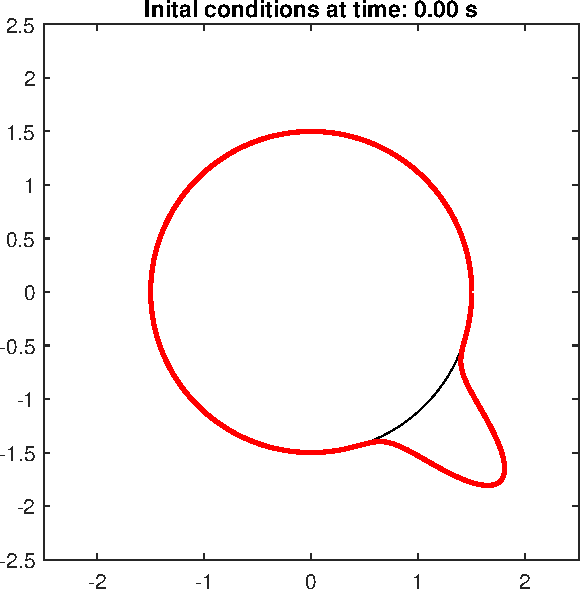
\includegraphics[width=0.4\textwidth]{C:/Users/Matteo/Shallow-Water-Equations/plots/SWE-spherical-1d-initial_conditions.pdf}
    \caption{Initial conditions for the 1D linearized shallow water equations in spherical coordinates.}\label{fig:swe_spherical_1d_initial_conditions}
\end{figure}



